\documentclass[UTF8,a4paper,11pt,fontset=fandol]{ctexart}

\usepackage[a4paper,margin=2.3cm]{geometry}
\usepackage{hyperref}
\usepackage{amsmath}
\usepackage{booktabs}
\usepackage{tikz}
\usepackage{graphicx}
\usepackage{xcolor}

% 待补数字：正文用 \TBD{...} 标出，定稿前替换为实测值并删除该命令。
\newcommand{\TBD}[1]{\textcolor{red}{[\,#1\,]}}

\title{数据分析}
\author{可视化导论第三次作业}
\date{2026年10月}

\hypersetup{colorlinks=true,linkcolor=blue,urlcolor=blue}

\begin{document}

\maketitle

\section{作品概述}

本次作业做了一个双语可视化数据分析工作台：中文入口 \url{https://vis.starlab.top/hw03/}，英文入口 \url{https://vis.starlab.top/en/hw03/}。它把筛选、清洗、统计、合并等八类数据分析操作做成图形界面，不写代码也能完成完整流程；熟悉 pandas 的读者则可以随时对照每一步对应哪个函数。

工作台按 pandas 常用 DataFrame 工作流分成整理、清洗、计算、统计、重塑、合并、索引、时间八个分区，共 59 个工具入口，支持用中文、英文或 pandas 函数名搜索。左侧是数据集、字段与操作时间线，中间是图形与数据表，右侧按当前工具出现参数区。

打开页面即可操作一份固定种子生成的教学合成零售数据：643 条订单与 6 条商品记录，故意留了重复记录和缺失成本。页面明确标注这是合成数据，不作为真实商业结论。

网站是纯静态前端：Astro 构建，TypeScript 写逻辑，D3 画图，没有后端；导入的数据与操作都留在浏览器里，不上传服务器。中文和英文共用同一套操作模型与状态，切换语言时数据集、筛选条件与历史步骤都保留（图~\ref{fig:theme}）。

\section{关键亮点}

\subsection{可视化分析：筛选、清洗、统计、合并等八类操作}

八个分区覆盖了从加载到分析的主要工作流，表~\ref{tab:coverage} 是各分区的代表能力与对应的 pandas 写法。筛选支持嵌套 AND/OR、集合与日期范围、位置与标签切片；清洗覆盖去重、缺失删除与填充插值；统计包含描述统计、分位数、频数以及 Pearson/Spearman 相关；合并支持多键的 left/inner/right/outer/cross 连接、拼接和就近关联；此外还有独立行索引与多层索引、透视与宽长表变形、字符串与日期处理、窗口重采样以及分箱抽样。

\begin{table}[!htbp]
  \centering
  \small
  \begin{tabular}{@{}lll@{}}
    \toprule
    分区 & 对应 pandas 工作流 & 可视化侧重点 \\
    \midrule
    整理 & 选列、rename、astype、sort、duplicated & 字段投影与类型徽标、批量命名前后映射 \\
    清洗 & dropna、fillna、interpolate、isin & 缺失矩阵、填充或删除的前后对比 \\
    计算 & assign、where、round、cut、sample & 公式依赖树、条件分支人数、分箱人数 \\
    统计 & describe、quantile、value\_counts、corr & 相关矩阵联动原始散点、箱线与 IQR \\
    重塑 & pivot\_table、crosstab、melt、stack & 拖拽行列键、热力矩阵、层级迁移图 \\
    合并 & merge、concat、merge\_asof & 字段配对、匹配率与未匹配键、位置映射 \\
    索引 & set/reset\_index、loc、reindex、MultiIndex & 标签格子、部分层重置、层级基数 \\
    时间 & to\_datetime、resample、rolling、ewm & 时间趋势、窗口权重曲线、增长率独立轴 \\
    \bottomrule
  \end{tabular}
  \caption{八个分区与 pandas 工作流的对应关系。}\label{tab:coverage}
\end{table}

最容易让人困惑的操作把诊断也一并画出来：合并之前给出两侧源记录的匹配率、输出行里两侧匹配与单侧记录的数量，以及优先列出的未匹配键分布（图~\ref{fig:explain} 右）；相关矩阵每格给出系数和有效配对数，点开单元格可以看到统计之前的原始配对散点（图~\ref{fig:explain} 左）。所有计算都基于完整数据，图形采样会明确标注，例如散点最多显示 1500 个点（图~\ref{fig:overview}）。

\subsection{即时预览：参数修改自动更新，支持前后对比}

改动任何参数都会自动重算预览，不需要先点按钮。结果区在“操作前 / 操作后 / 对比”之间切换，上方摘要直接写出这一步对数据的影响——图~\ref{fig:preview} 中字段数 $9 \rightarrow 10$、缺失值 $23 \rightarrow 46$。对比视图把操作前后的分布画在共用刻度上，并优先使用当前操作涉及的数值字段；默认视图按结果区宽度选择，手动选定的视图在继续调整参数时保留。

只有预览有效时“应用操作”才可点击，参数不合法会先被拦住；提交计算期间修改控件被锁定，过期请求按序号丢弃，旧结果不会盖住新参数。公式、条件赋值这类计算还会给出依赖树、分支人数和逐行的原文与结果对照，确认之后才写入数据。

\subsection{图表联动：点击、框选图表即可筛选数据}

分布直方图、类别柱形和关系散点不只是展示。点击柱形按区间或类别筛选，在散点上拖动框选记录，都会生成一条可编辑、可删除的筛选条件标签，并和数据表、字段摘要同步更新（图~\ref{fig:overview}）。

探索和提交分开：点选先形成“临时选择”，只有点“应用筛选”才写入操作时间线，误点不会污染分析链；排除匹配是同一入口的反向操作。筛选生效后图表仍以灰色保留全量分布，读者看得见“筛掉了什么”，不会失去参照。查看预览或历史步骤时，图形不会直接改动数据。

\subsection{过程可追溯：时间线、撤销重做、本地自动保存}

每一步操作都进入时间线，记录参数、输入输出行列数和结果说明，可以随时回看。撤销与重做之外，从旧步骤继续会产生一条可切换的分支，原来的分析链保留可恢复；多个数据集各有独立时间线，切换数据集不会串味。

工作状态自动保存在浏览器本地：原始文件和操作步骤分开存进 IndexedDB，原始内容按 SHA-256 去重，工作区只记录数据集引用与操作序列，解析后的整张表不重复落盘，快照不会随历史版本线性膨胀。写入带版本检查，另一个标签页更新过就拒绝覆盖并提示先备份；刷新或重开页面会重新解析原始文件并重放时间线，不需要重新选择文件。存储面板可以开关自动保存、查看配额占用、清除本站数据或下载备份。

\subsection{支持多格式导入、结果导出与离线重放}

导入支持 CSV、TSV、对象数组 JSON、XLSX（可选工作表）和 Parquet（六种压缩、LIST 列表），也可以从公开 URL 读取；分隔符与编码可选，带前导零的标识符按文本保留，解析在 Worker 中执行，格式出错会指出具体位置而不是静默丢行。

导出分三级：当前结果导 CSV 或 JSON，整个工作区导 JSON 备份（含原始文件、操作与视图配置），以及自包含的 Node.js 离线重放脚本——脚本内嵌操作引擎和被引用的原始数据，不打开网站也能重算出同一份结果。同一套操作还能导出 Python 脚本，文中明确说明它是桥接脚本：先重放引擎，再恢复 pandas 的行列索引、可空列与分类类型，而不是把每一步翻译成原生 pandas 调用。

\section{页面截图}

图~\ref{fig:overview} 与图~\ref{fig:preview} 取自当前版本的 1440$\times$1000 视口；图~\ref{fig:explain} 的两张功能截图取自界面精简前的版本，功能与当前版本一致，页头已裁去；图~\ref{fig:theme} 为英文深色主题与 390\,px 窄屏。

\begin{figure}[!htbp]
  \centering
  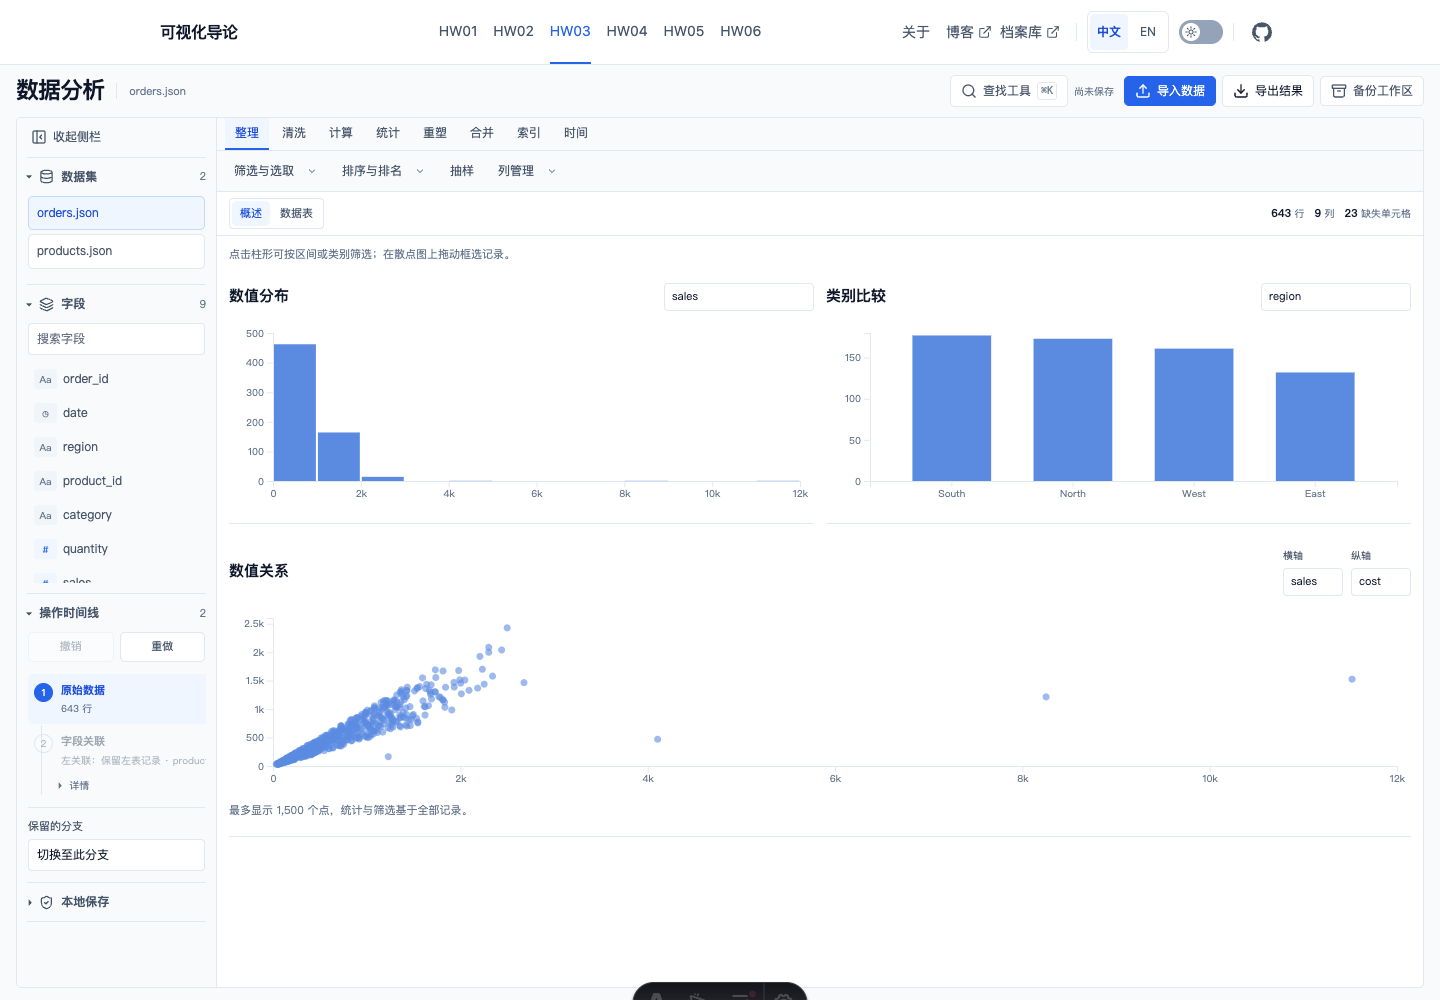
\includegraphics[width=0.78\textwidth]{images/overview-light.png}
  \caption{工作台总览。左侧是数据集、字段与操作时间线，中间是数值分布、类别比较和数值关系三张联动图，右侧在选中工具后出现参数区。默认数据 643 行、9 列、23 个缺失单元格。}
  \label{fig:overview}
\end{figure}

\begin{figure}[!htbp]
  \centering
  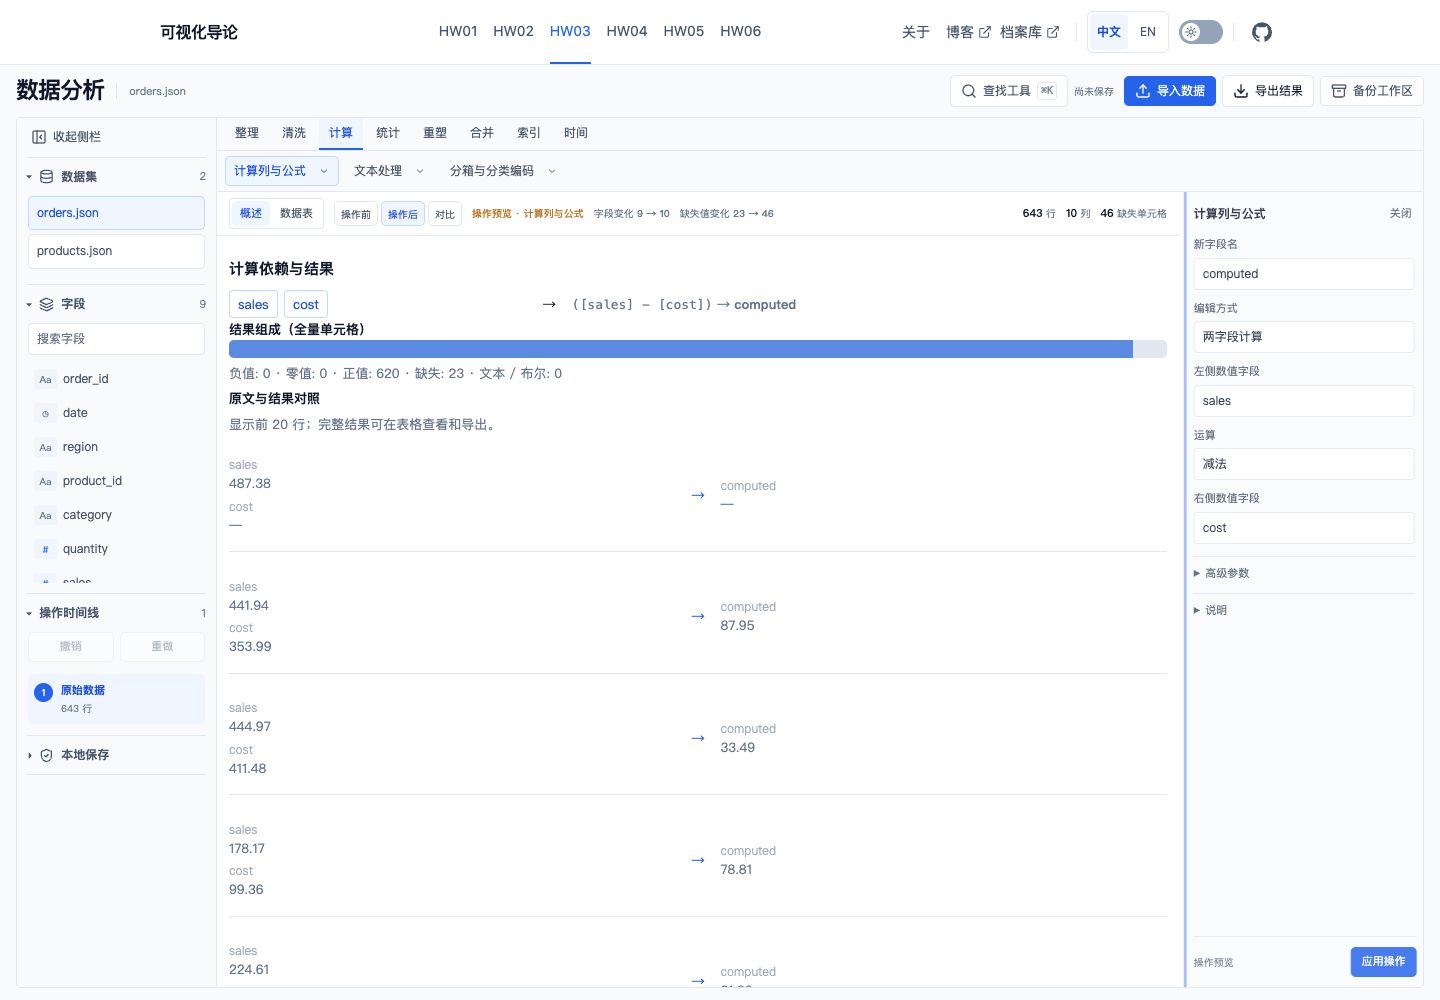
\includegraphics[width=0.78\textwidth]{images/preview-formula.png}
  \caption{即时预览与公式解释。结果区可在“操作前 / 操作后 / 对比”之间切换，摘要写出字段数与缺失值的变化；公式以依赖树呈现，配合结果组成和逐行原文与结果对照，确认后再点“应用操作”。}
  \label{fig:preview}
\end{figure}

\begin{figure}[!htbp]
  \centering
  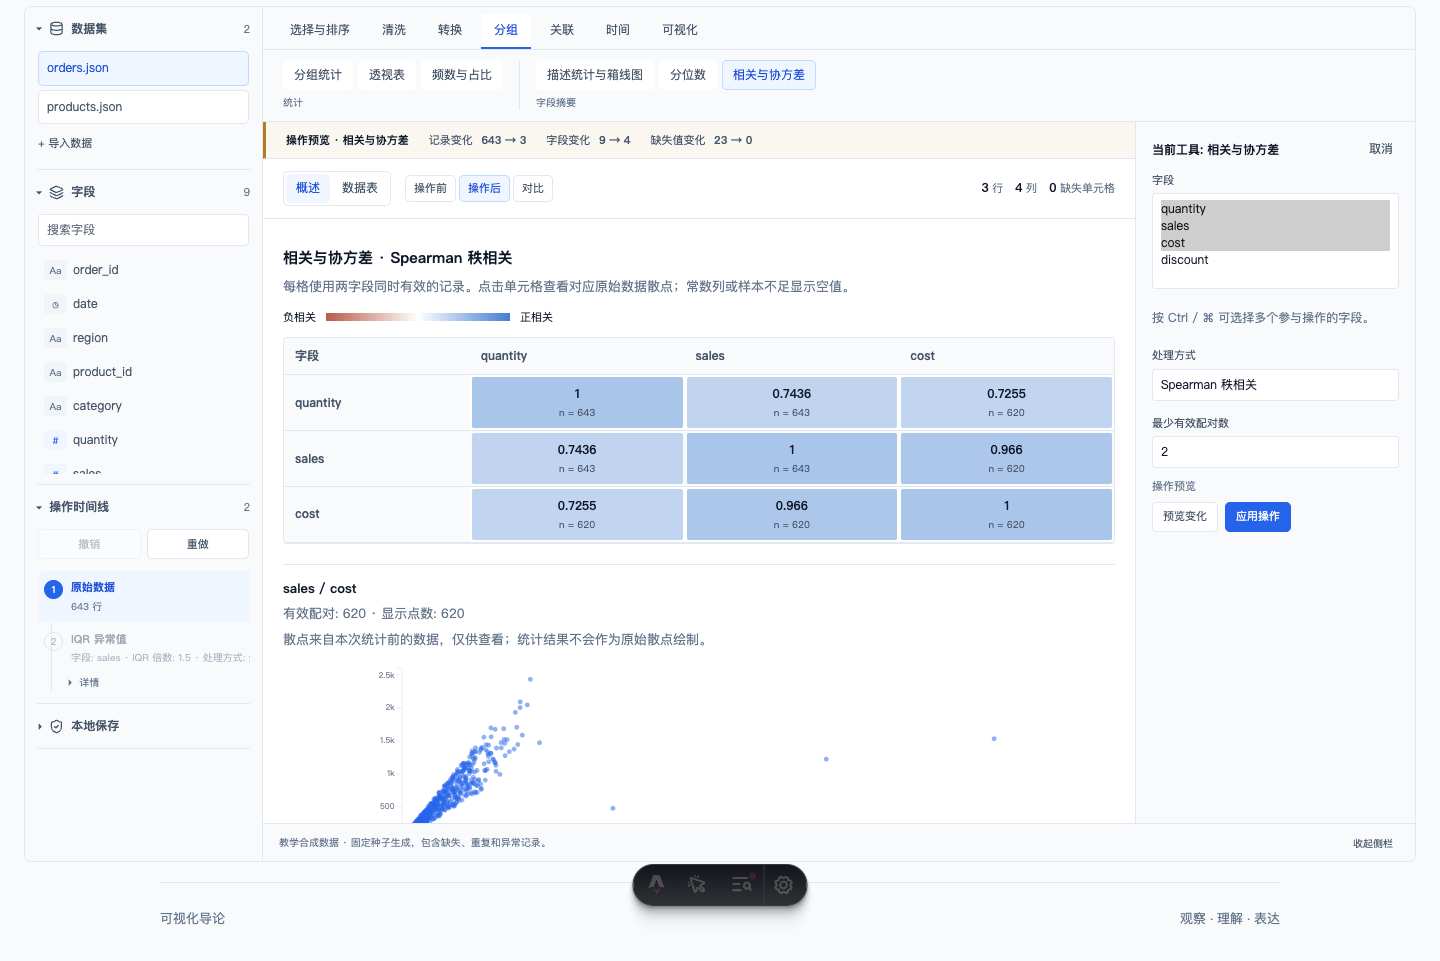
\includegraphics[width=0.487\textwidth]{images/correlation-scatter.png}\hfill
  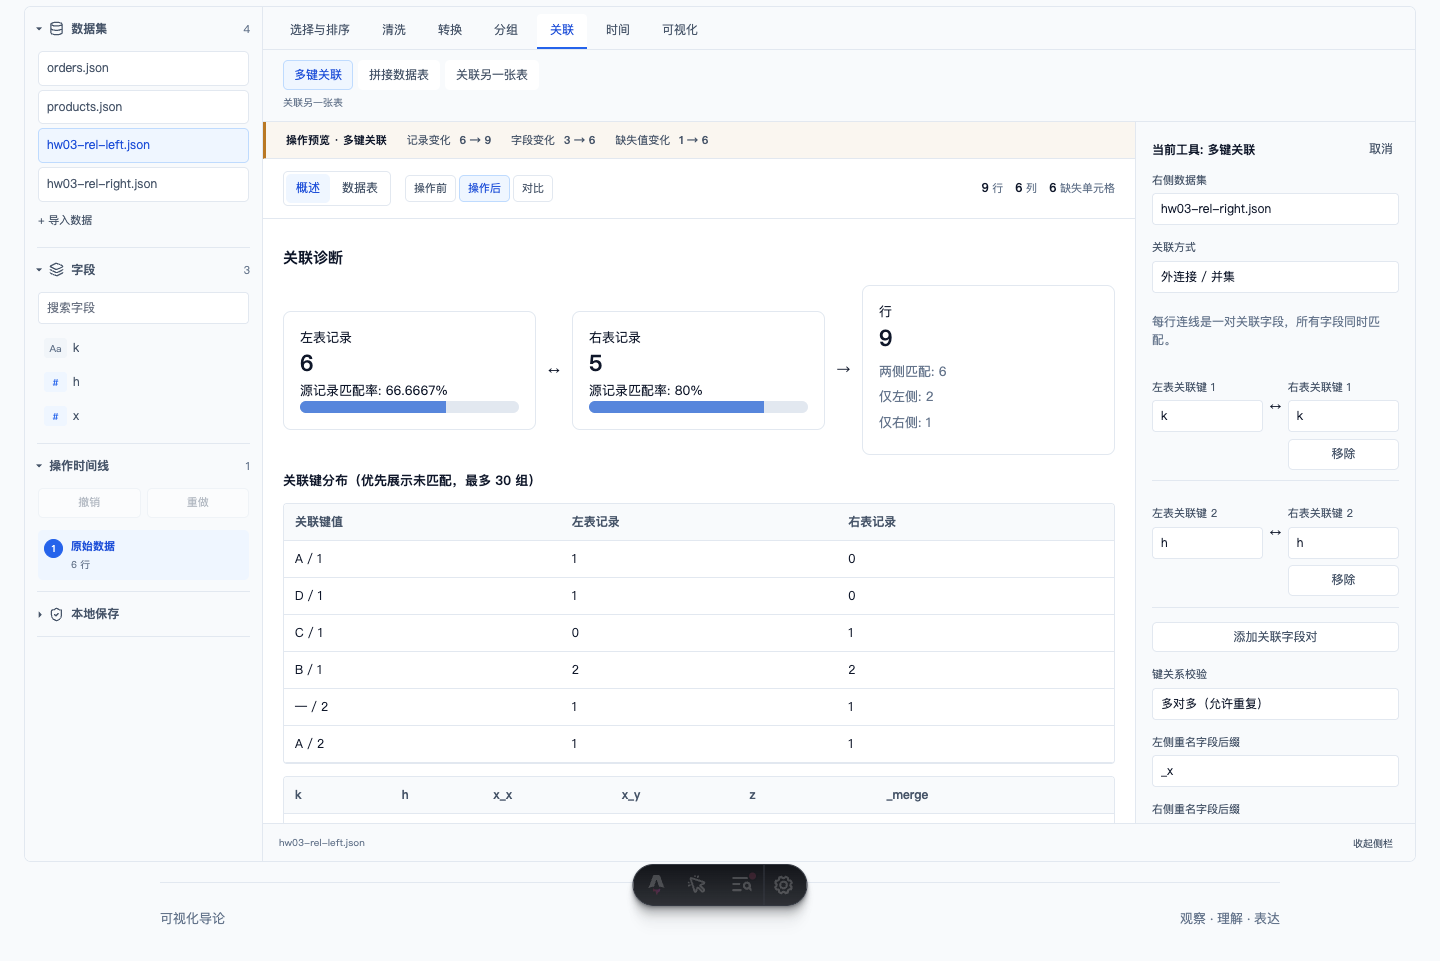
\includegraphics[width=0.487\textwidth]{images/join-diagnostics.png}
  \caption{左：相关与协方差矩阵，每格给出系数和有效配对数，点开单元格可以看到统计前的原始配对散点。右：多键外连接的诊断，显示两侧源记录匹配率、输出中两侧匹配与单侧记录数量，以及优先列出的未匹配键分布。}
  \label{fig:explain}
\end{figure}

\begin{figure}[!htbp]
  \centering
  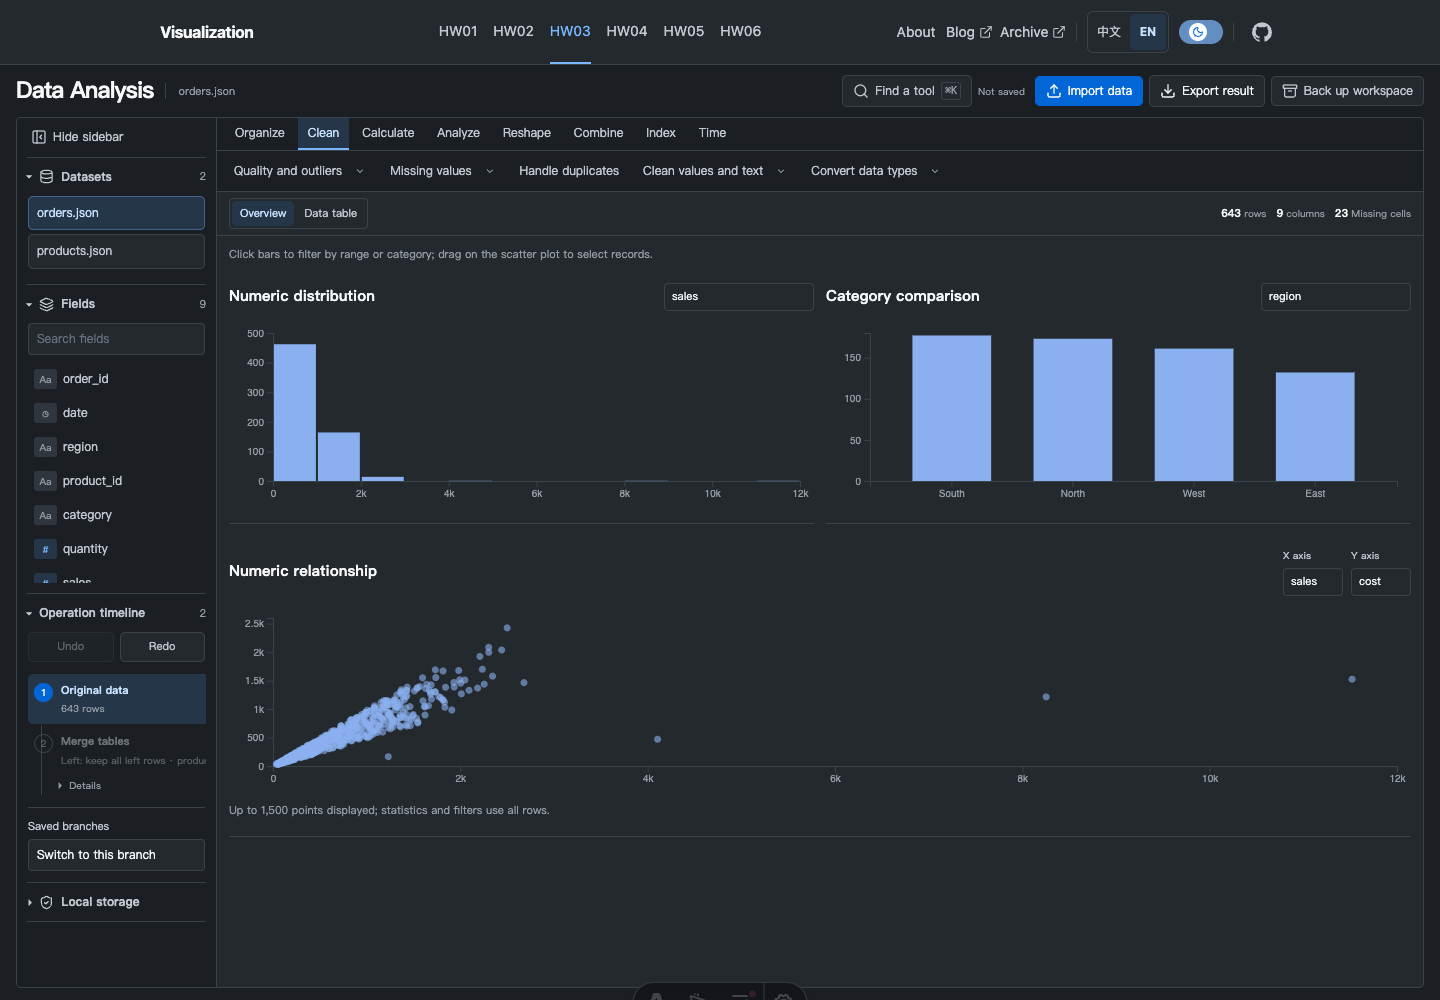
\includegraphics[height=5.2cm]{images/english-dark.png}\hfill
  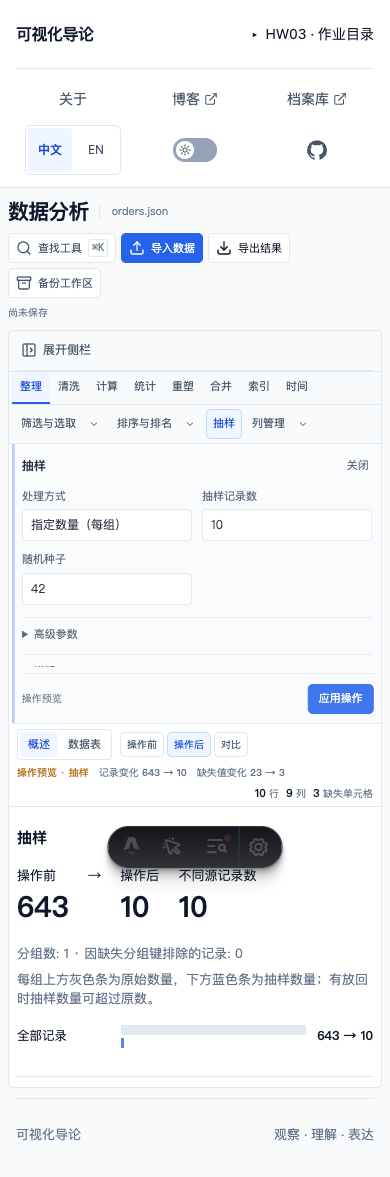
\includegraphics[height=5.2cm]{images/mobile-390.png}
  \caption{左：英文界面与深色主题，工具名、图表标题和说明整体切换，分析状态不变。右：390\,px 窄屏下的抽样工具，参数区与预览叠放，摘要显示 643 行抽样为 10 行。}
  \label{fig:theme}
\end{figure}

\end{document}
